% Created 2025-12-16 Tue 20:04
% Intended LaTeX compiler: pdflatex
\documentclass[11pt]{article}
\usepackage[utf8]{inputenc}
\usepackage[T1]{fontenc}
\usepackage{graphicx}
\usepackage{longtable}
\usepackage{wrapfig}
\usepackage{rotating}
\usepackage[normalem]{ulem}
\usepackage{amsmath}
\usepackage{amssymb}
\usepackage{capt-of}
\usepackage{hyperref}
\usepackage{mathptmx}  % Times font
\usepackage{helvet}   % Helvetica font
\renewcommand{\familydefault}{\sfdefault} % Sans-serif as default
\usepackage{titlesec}
\usepackage{lmodern}
\usepackage{tikz}
\usepackage{pgfplots}
\pgfplotsset{compat=1.18}
\author{Serob Tigranyan}
\date{\today}
\title{Matematical Analysis}
\hypersetup{
 pdfauthor={Serob Tigranyan},
 pdftitle={Matematical Analysis},
 pdfkeywords={},
 pdfsubject={},
 pdfcreator={Emacs 30.2 (Org mode 9.7.34)}, 
 pdflang={English}}
\begin{document}

\maketitle
\tableofcontents

\newpage
\section{Calculate Area under Curve}
\label{sec:orgc7f3643}
Find the are under the cruve bounded by \(y=8+2x-x^2\) \& \(2x-y+4=0\).
\subsection{Finding Points of Intersection}
\label{sec:orgded6d20}
To find the area between the curves, we first need to determine where they intersect. We set the two equations equal to each other:
\[
8+2x-x^2=2x+4
\]
Simplifying:
\[
8+2x-x^2=2x+4
\]
\[
8-x^2=4
\]
\[
-x^2=-4
\]
\[
x^2=4 
\]

Therefore:
\[
x=\pm 2
\]

The curves intersect at \(x=-2\) and \(x=2\).

\newpage
\subsection{Graphical Representation}
\label{sec:orge1e3d3e}
The shaded region represents the area to be calculated between the parabola and the line.

\begin{center}
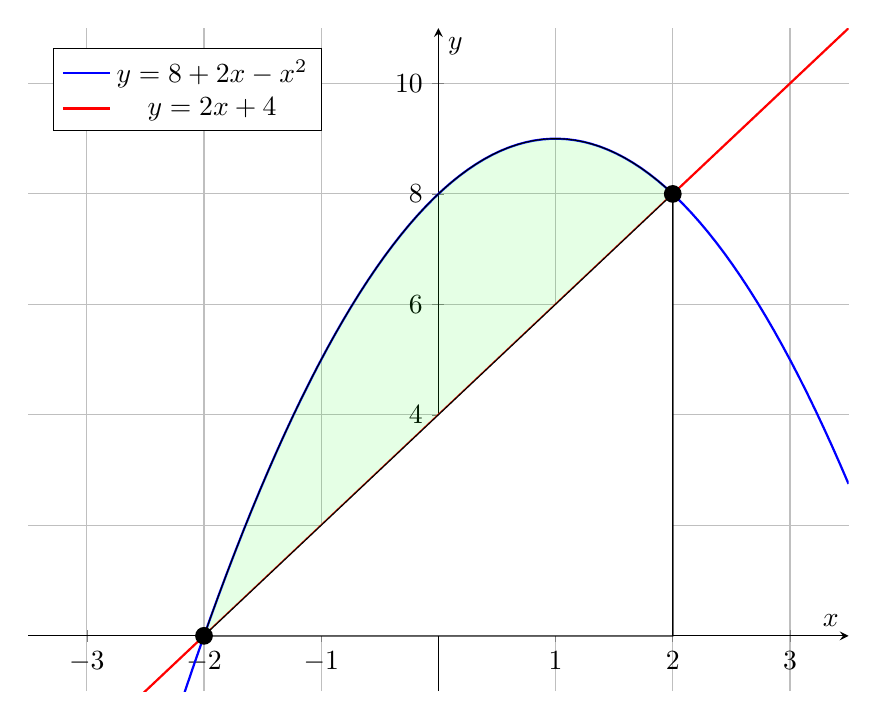
\begin{tikzpicture}
\begin{axis}[
    axis lines = center,
    xlabel = $x$,
    ylabel = $y$,
    xmin=-3.5, xmax=3.5,
    ymin=-1, ymax=11,
    width=12cm,
    height=10cm,
    grid=major,
    legend pos=north west,
]

% Plot the parabola
\addplot[
    domain=-3.5:3.5,
    samples=100,
    color=blue,
    thick,
]
{8+2*x-x^2};
\addlegendentry{$y=8+2x-x^2$}

% Plot the line
\addplot[
    domain=-3.5:3.5,
    samples=50,
    color=red,
    thick,
]
{2*x+4};
\addlegendentry{$y=2x+4$}

% Fill the area between curves
\addplot[
    fill=green,
    fill opacity=0.1,
    domain=-2:2,
    samples=100,
] {8+2*x-x^2} \closedcycle;

\addplot[
    fill=white,
    fill opacity=1,
    domain=-2:2,
    samples=50,
] {2*x+4} \closedcycle;

% Mark intersection points
\addplot[only marks, mark=*, mark size=3pt, color=black] coordinates {(-2,0) (2,8)};

\end{axis}
\end{tikzpicture}
\end{center}

\newpage
\subsection{Computing the Area}
\label{sec:org33c199f}
The area between two curves is computed by subtracting the area under the lower curve from the area under the upper curve:
\[
S_1 - S_2
\]
\[
S_1 = \int_{-2}^{2}{8+2x-x^2}dx = \left[ 8x+x^2-\frac{x^3}{3} \right]_{-2}^{2} = \frac{80}{3}
\]
\[
S_2 = \int_{-2}^{2}{2x+4}dx = \left[ x^2+4x \right]_{-2}^{2} = 16
\] 
\[
S_1 - S_2 = \boxed{ \frac{32}{3} }
\]

\newpage
\section{Show that function satisfies the given formula}
\label{sec:org6751ac3}
Given the function:
\[
z = \ln{x^2+xy+y^2}
\]
Show that this function satisfies the formula below:
\[
x\frac{\partial z}{\partial x} + y\frac{\partial z}{\partial y} = 2
\]

To verify this, we'll compute both partial derivatives and plug them into the formula.
\subsection{Differentiate function for x}
\label{sec:org772df57}
We apply the chain rule to find the partial derivative with respect to \(x\):
\[
\frac{\partial }{\partial x} \ln{x^2+xy+y^2} = \frac{\partial (x^2+xy+y^2)}{\partial x} \cdot \frac{1}{x^2+xy+y^2} = \frac{2x+y}{x^2+xy+y^2}
\]
\subsection{Differentiate function for y}
\label{sec:org95ad123}
Similarily:
\[
\frac{\partial }{\partial y} \ln{x^2+xy+y^2} = \frac{x+2y}{x^2+xy+y^2}
\]
\subsection{Plugging back to the formula}
\label{sec:org6743bf1}
Now we substitute the partial derivatives into the original formula and simplify:
\[
x\frac{2x+y}{x^2+xy+y^2} + y\frac{x+2y}{x^2+xy+y^2} = \frac{x(2x+y)+y(x+2y)}{x^2+xy+y^2}
\]
\[
= \frac{2x^2+xy+yx+2y^2}{x^2+xy+y^2}=\frac{2x^2+2xy+2y^2}{x^2+xy+y^2}= \frac{2(x^2+xy+y^2)}{x^2+xy+y^2} = \boxed{2}
\]

\newpage
\section{Find Convergence/Divergence of the given Series}
\label{sec:orgb81d399}
Given the Series:
\[
\sum_{n=1}^{\infty}{\frac{1}{\sqrt{n(n+1)}}}
\]
Find wether or not this series converges or diverges.
\subsection{Find a similar series to compare to}
\label{sec:orgfb58af3}
We use the limit comparison test. Because as \(n\) grows larger, \(\frac{1}{\sqrt{n(n+1)}}\) behaves similarly to \(\frac{1}{n}\), we choose:
\[
\sum_{n=1}^{\infty}{\frac{1}{n}}
\]

First, we verify that this comparison series diverges using the integral test:
\[
\int_{1}^{\infty}{\frac{1}{x}dx} = \left[ \ln{\left| x\right|} \right]_{1}^{\infty} = \infty
\]

Since the integral diverges, the harmonic series \(\sum_{n=1}^{\infty}{\frac{1}{n}}\) also diverges.
\subsection{Limit comparison test}
\label{sec:org5bd1235}
We compute the limit of the ratio of the two series:
\[
\lim_{n\to\infty}{\frac{a_n}{b_n}} = L
\]
\[
\lim_{n\to\infty}{ \frac{\frac{1}{\sqrt{n(n+1)}}}{\frac{1}{n}} } = \lim_{n\to\infty}{ \frac{n}{\sqrt{n(n+1)}} } = \lim_{n\to\infty}{ \frac{n}{\sqrt{n^2(1+\frac{1}{n})}} } = \lim_{n\to\infty}{\frac{n}{n\sqrt{1+\frac{1}{n}}}} = \frac{1}{\sqrt{1 + 0}} = 1
\]

Since the limit equals a positive constant, both series share the same convergence behavior. Because \(\sum_{n=1}^{\infty}{\frac{1}{n}}\) diverges, we conclude:
\[
\boxed{\sum_{n=1}^{\infty}{\frac{1}{\sqrt{n(n+1)}}} \text{ diverges}}
\]
\end{document}
